\subsection{Adhesion of Metal Oxide Interfaces}
\begin{frame}{
    Adhesion in FeBCC/Fe\textsubscript{3}O\textsubscript{4}
    interface 
  }

  \begin{onlyenv}<1>
    Separating the parts of the interface it is
    possible to obtain energy vs separation curves 
    from DFT calculations.
    Then the forces can be obtained from interface 
    potential models!
  \end{onlyenv}
  \begin{center}
  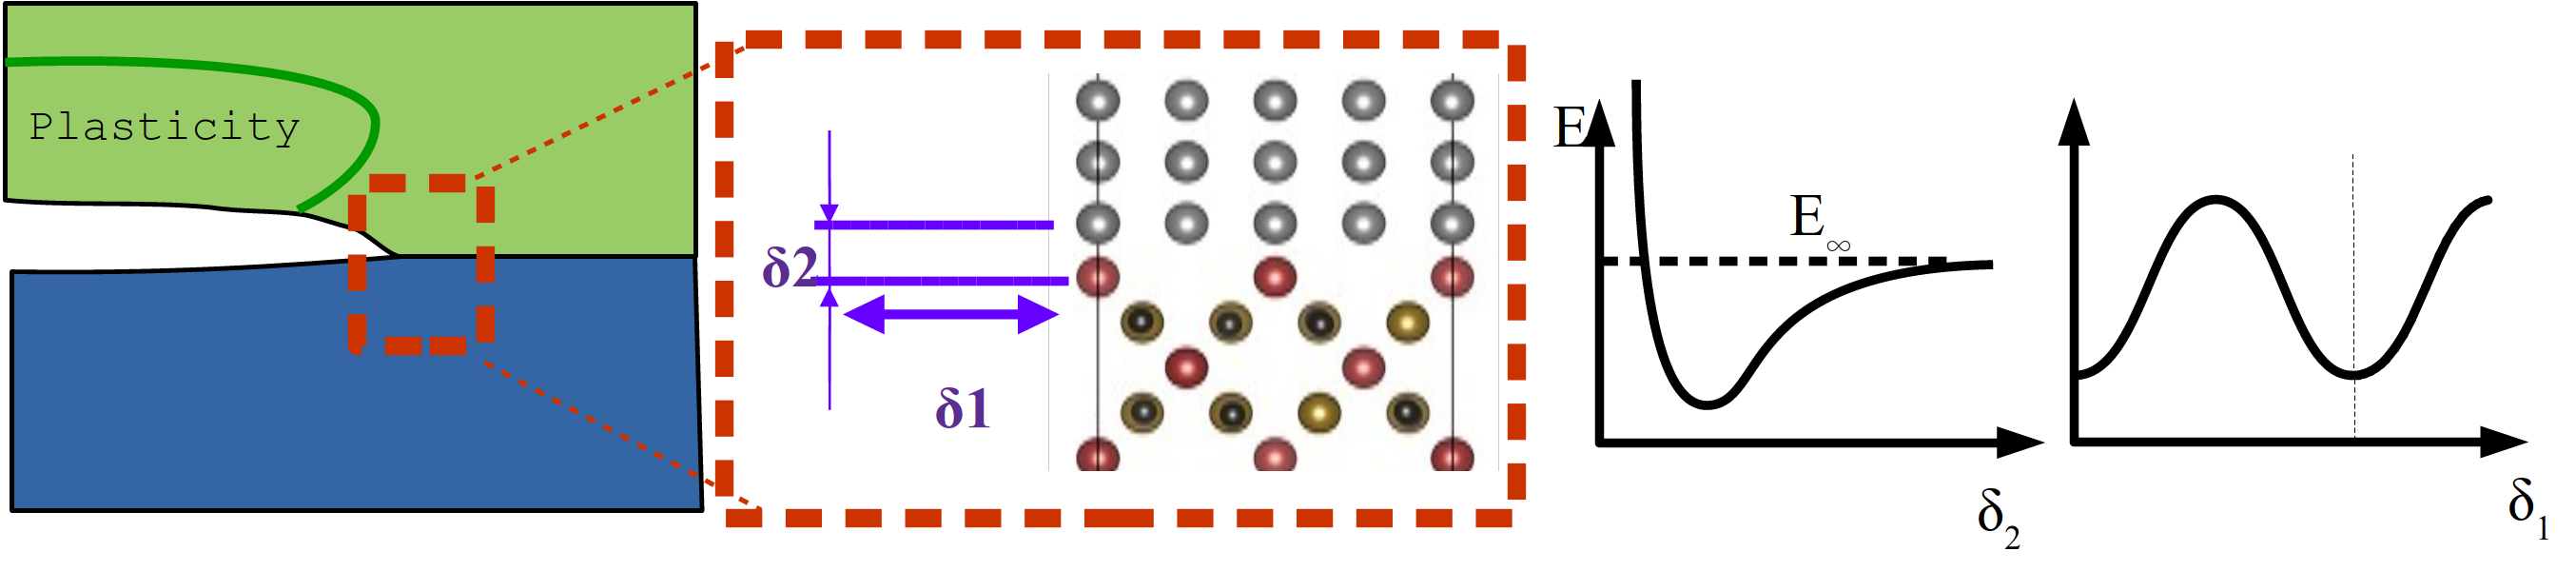
\includegraphics[width=\textwidth]{/home/mariano/CuadernoTrabajo/CV/SLI/02-CurrentResearch/Adhesion_Scheme.png}
  \end{center}

    \begin{onlyenv}<2->

\begin{align*}
  \resizebox{!}{0.5\height}{$
  \tilde{L}_{\delta_1}{}={}
  \frac{E_{ad}}{W_{sep}}{}={}
  \exp{\left(  \frac{\delta_2}{\hat{\delta} } \right)}
  \sum_{i=0} ^{i_{max}} \left(1 + \beta \right) ^i
   \left[ -1 + 
   f (\delta_1) \left( 1 + \beta \right) ^i
   \right]
   \alpha _i
   \left(
   \frac{\delta_2}{\hat{\delta}}
   \right) ^i \quad $}
   &
   \quad
  \resizebox{!}{0.5\height}{$
   T_1 \left(\delta_1
   ,\delta_2 \right) = - \frac{\partial W}{\partial \delta _1}
   \quad
   $}
   &
  \resizebox{!}{0.5\height}{$
   \quad
   T_2 \left(\delta_1 ,\delta_2 \right) = -\frac{\partial W}{\partial \delta_2}
   \quad
   $}
\end{align*}
%\alpha _i 
%\left( 
%\left{\frac{\delta_2}{\hat{\delta}}\right}\right) ^i
%\end{equation}
%
  \begin{columns}
    \column{0.5\textwidth}
  \begin{center}
    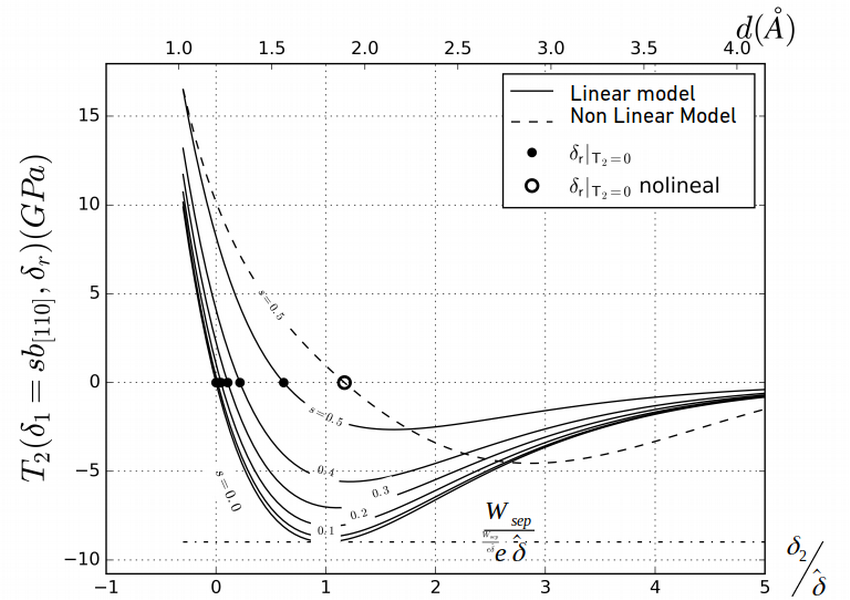
\includegraphics[height=3cm]{/home/mariano/CuadernoTrabajo/CV/SLI/02-CurrentResearch/T1.png}
  \end{center}
    \column{0.5\textwidth}
  \begin{center}
    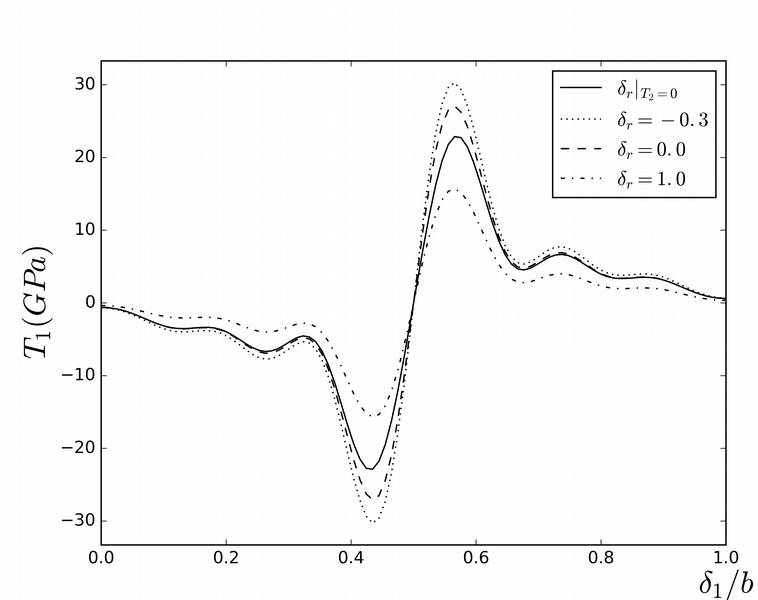
\includegraphics[height=3cm]{/home/mariano/CuadernoTrabajo/CV/SLI/02-CurrentResearch/T2.png}
  \end{center}
  \end{columns}
\end{onlyenv}
\end{frame}
